%------------------------------------------%
% Saturday Morning Statistics
% Date: 12/11/2021
%------------------------------------------%
\documentclass[xcolor={dvipsnames}]{beamer}
\hypersetup{pdfpagemode=FullScreen}
\mode<presentation>{
  \usetheme{Boadilla}
  \usecolortheme{orchid}
  \usefonttheme{default}
  \setbeamertemplate{navigation symbols}{}
  \setbeamertemplate{caption}[numbered]
} 
\usepackage[english]{babel}
\usepackage[utf8x]{inputenc}
\setbeamersize{text margin left=0.5in,text margin right=0.5in}

\usepackage[dvipsnames]{xcolor}
\definecolor{DarkGreen}{RGB}{2, 48, 32}
\definecolor{CalyxGreen}{RGB}{34, 153, 84}
\definecolor{DarkOrange}{RGB}{199, 0, 57}
\definecolor{LightOrange}{RGB}{255, 87, 51}
\definecolor{LightGreen}{RGB}{218, 247, 166}
\definecolor{LightYellow}{RGB}{255, 195, 0}

\setbeamercolor*{palette primary}{bg=LightGreen, fg = DarkGreen}
\setbeamercolor*{palette secondary}{bg=LightGreen, fg=DarkGreen}
\setbeamercolor*{palette tertiary}{bg=LightGreen, fg = DarkGreen}
%\setbeamercolor*{palette quaternary}{bg=myNewColorD, fg = green}

%------------------------------------------%
% Packages
%------------------------------------------%
\usepackage{amsmath}
\renewcommand*\footnoterule{} %No sperating line on footnote
\usepackage{mathtools} %ANNOTATING EQUATIONS
\usepackage{hhline} %DOUBLBARS
\usepackage[super]{nth}
\usepackage{graphicx, caption, subcaption}

%------------------------------------------%
% Commands
%------------------------------------------%
\newcommand\T{\rule{0pt}{2.5ex}} %TOPSTRUT
\newcommand\B{\rule[-1.25ex]{0pt}{0pt}} %BOTTOMSTRUT
\newenvironment<>{varblock}[2][.9\textwidth] %RESIZED BLOCKS
  {\setlength{\textwidth}{#1}
  \begin{actionenv}#3
    \def\insertblocktitle{#2}\par
    \usebeamertemplate{block begin}}
  {\par\usebeamertemplate{block end}
  \end{actionenv}}
\defbeamertemplate{enumerate item}{largeball} %LARGE BALLS
{\begin{pgfpicture}{-1ex}{-0.65ex}{1.5ex}{1.5ex}
\usebeamercolor[fg]{item projected}
{\pgftransformscale{2.5}\pgftext{\Large\pgfuseshading{bigsphere}}}
{\pgftransformshift{\pgfpoint{0pt}{0.5pt}}
\pgftext{\usebeamerfont*{item projected}\small\insertenumlabel}}
\end{pgfpicture}}
\usepackage{tikz} % FANCY ARROWS
\usepackage{xparse}
\NewDocumentCommand\UpArrow{O{2.0ex} O{black}}{%
   \mathrel{\tikz[baseline] \draw [->, line width=0.5pt, #2] (0,0) -- ++(0,#1);}} % FANCY UPARROW
\NewDocumentCommand\DownArrow{O{2.0ex} O{black}}{%
   \mathrel{\tikz[baseline] \draw [<-, line width=0.5pt, #2] (0,0) -- ++(0,#1);}} % FANCY DOWNARROW
%\vskip 1cm
\makeatletter
\newcommand{\LeftEqNo}{\let\veqno\@@leqno}%LEFT EQUATION #'s
\makeatother

%------------------------------------------%
% Title
%------------------------------------------%
\title[\textbf{Saturday Morning Statistics}]{}
\author{Cannabis Data Science}
\institute[]{\Large Saturday Morning Statistics}
\date{December \nth{11}, 2021}
\begin{document}
\begin{frame}{}
  
\includegraphics[scale=0.075]{images/logos/cannlytics_logo_with_text_light.png}
  \titlepage
\end{frame}

%------------------------------------------%
% Introduction
%------------------------------------------%

\section{Introduction}

%------------------------------------------%
% Quantity caps.
%------------------------------------------%

\begin{frame}{}

{\large \textbf{Who bears the cost of quantity restrictions?}}\vspace{0.5\baselineskip}\\

\begin{figure}
    \begin{subfigure}[t]{.4\textwidth}
      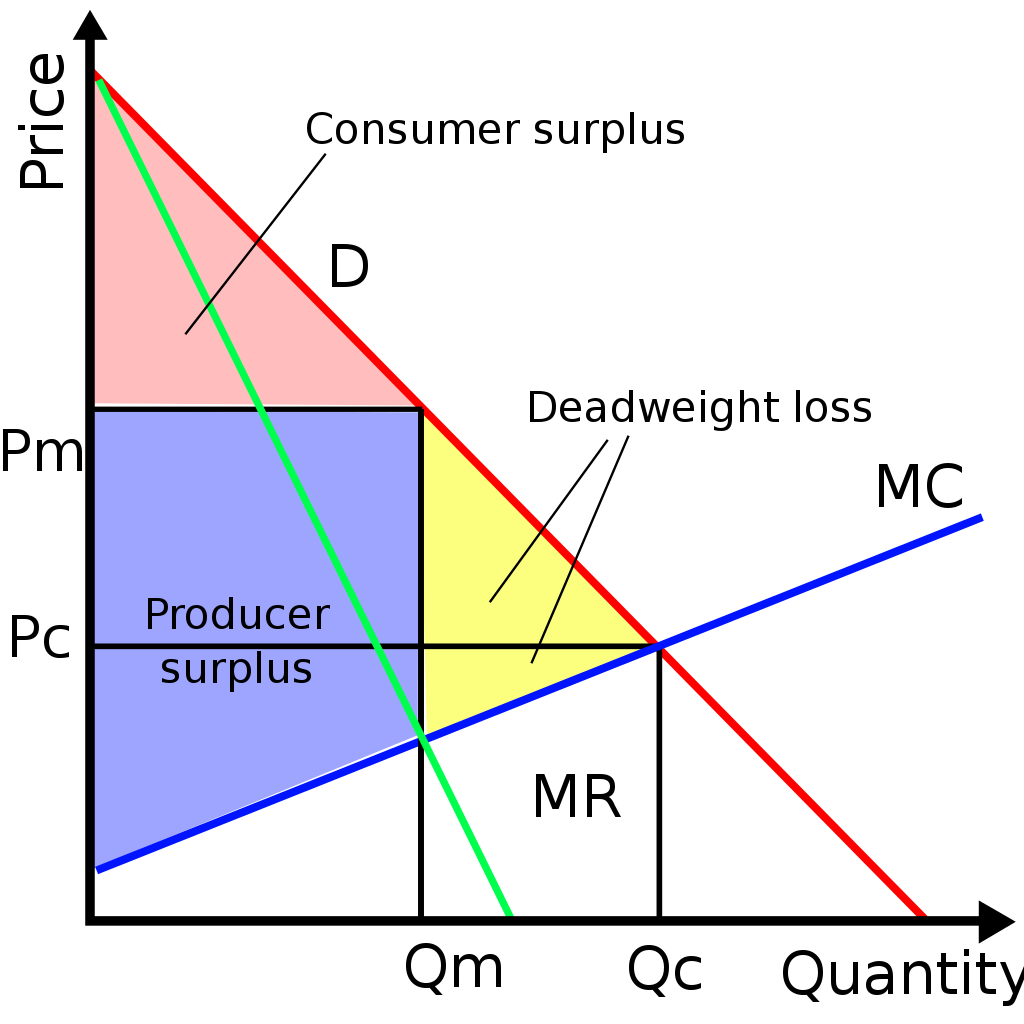
\includegraphics[width=\textwidth]{images/monopoly-surpluses.png}
      \caption*{\scriptsize Effects of a quantity restrictions on a market\newline\tiny Source: 	SilverStar at en.wikipedia}
    \end{subfigure}
\end{figure}

\vspace{0.5\baselineskip}{\large It depends...!}

\end{frame}

%------------------------------------------%
% The identification problem
%------------------------------------------%

\begin{frame}{}

{\large \textbf{The identification problem}}\vspace{0.5\baselineskip}\\

\begin{figure}
    \begin{subfigure}[t]{.4\textwidth}
      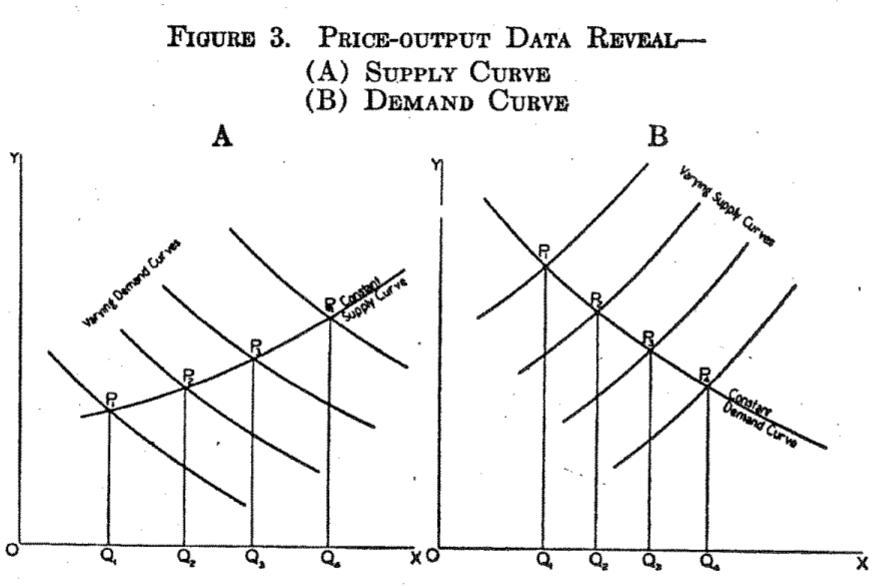
\includegraphics[width=\textwidth]{images/supply-and-demand-shifts-vegetable-oil.png}
      \caption*{\tiny The Tariff on Animal and Vegetable Oils by Phillip G. Wright (1928)\tiny \newline Retrieved from: https://scholar.harvard.edu}
    \end{subfigure}\hspace{.5in}%
    \begin{subfigure}[t]{.4\textwidth}
      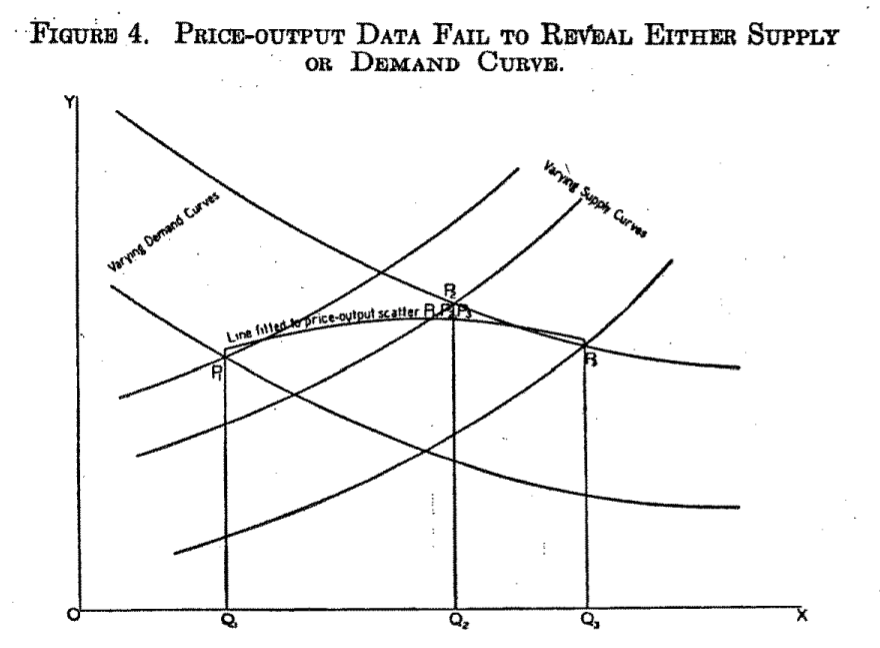
\includegraphics[width=\textwidth]{images/supply-and-demand-identification-problem-vegetable-oil.png}
      \caption*{\tiny The Tariff on Animal and Vegetable Oils by Phillip G. Wright (1928)\tiny \newline Retrieved from: https://scholar.harvard.edu}
    \end{subfigure}
\end{figure}

\vspace{0.5\baselineskip}{\large The change in price and quantity depends...!}

\end{frame}

%------------------------------------------%
% Instrumental variables meme
%------------------------------------------%

\begin{frame}{}

{\large \textbf{We need a cannabis supply IV, STAT!}}\vspace{0.5\baselineskip}\\

\begin{figure}
    \begin{subfigure}[t]{0.5\textwidth}
      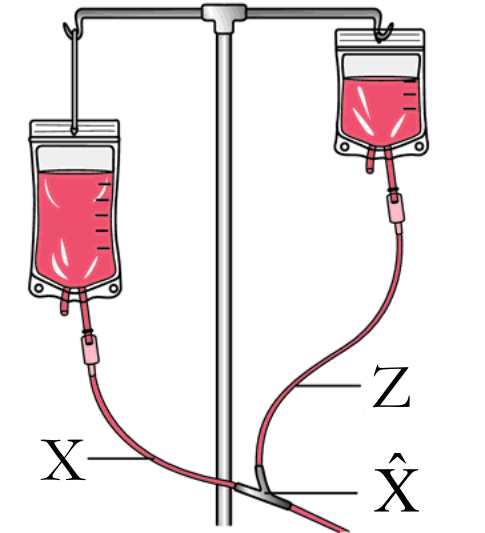
\includegraphics[width=\textwidth]{images/iv-meme.png}
    \end{subfigure}
\end{figure}

\end{frame}

%------------------------------------------%
% Why do we need IVs?
%------------------------------------------%

\begin{frame}{}

{\large \textbf{Why do we need an IV?}}\vspace{1\baselineskip}\\

\begin{itemize}

\item \textbf{Reverse causation} -- changes in the dependent variable change the value of at least one of the independent variables.
\vspace{1\baselineskip}\\
\item \textbf{Omitted variables} -- there are variables that affect both the dependent and independent variables that are not included in the model.
\vspace{1\baselineskip}\\
\item \textbf{Measurement error} -- the independent variables are subject to non-random measurement error.

\end{itemize}

\end{frame}

%------------------------------------------%
% Problems with Endogeneity
%------------------------------------------%

\begin{frame}{}

{\large \textbf{What happens if we don't use an IV?}}\vspace{1\baselineskip}\\

\begin{itemize}

\item Our explanatory (independent) variables may be endogenous.
\vspace{1\baselineskip}\\
\item If our explanatory variables are endogenous, then any OLS estimates are biased and inconsistent.

\end{itemize}

\end{frame}

%------------------------------------------%
% Good IVs
%------------------------------------------%

\begin{frame}{}

{\large \textbf{What makes a good IV?}}\vspace{1\baselineskip}\\

\begin{enumerate}

\item The instrument must be correlated with the endogenous explanatory variable(s). The more correlated the better.
\vspace{1\baselineskip}\\
\item The instrument cannot be correlated with the error term in the explanatory equation. This is the \textbf{exclusion restriction}.

\end{enumerate}

\end{frame}

%------------------------------------------%
% Possible IVs
%------------------------------------------%

\begin{frame}{}

{\large \textbf{What variables can we use as an IV?}}\vspace{1\baselineskip}\\

\begin{enumerate}

\item Energy prices?
\vspace{1\baselineskip}\\
\item Changes in labor supply?
\vspace{1\baselineskip}\\
\item Building material prices?
\vspace{1\baselineskip}\\
\item Real estate prices?

\end{enumerate}

\end{frame}

%------------------------------------------%
% Future work
%------------------------------------------%

\begin{frame}

{\large \textbf{Future work}: Start preparing forecasts for 2022!}\vspace{1\baselineskip}\\

\begin{enumerate}

\item Supply chain factors.
\vspace{1\baselineskip}\\
\item Inflation.
\vspace{1\baselineskip}\\
\item Domestic spending.
\vspace{1\baselineskip}\\
\item Employment

\end{enumerate}

\end{frame}

%------------------------------------------%
% Takeaway
%------------------------------------------%

\begin{frame}{}

\begin{center}
\begin{minipage}{3.85in}


\includegraphics[width=.25in]{images/prayer.png} {\Large \textbf{Thank you for coming.}}\vspace{0.5\baselineskip}\\

Take some time and discuss any conclusions drawn.

\end{minipage}
\end{center}

\end{frame}

%------------------------------------------%
% Finale
%------------------------------------------%
\end{document}
